\documentclass{standalone}
\usepackage{tikz}
\usetikzlibrary{patterns, positioning}

\begin{document}
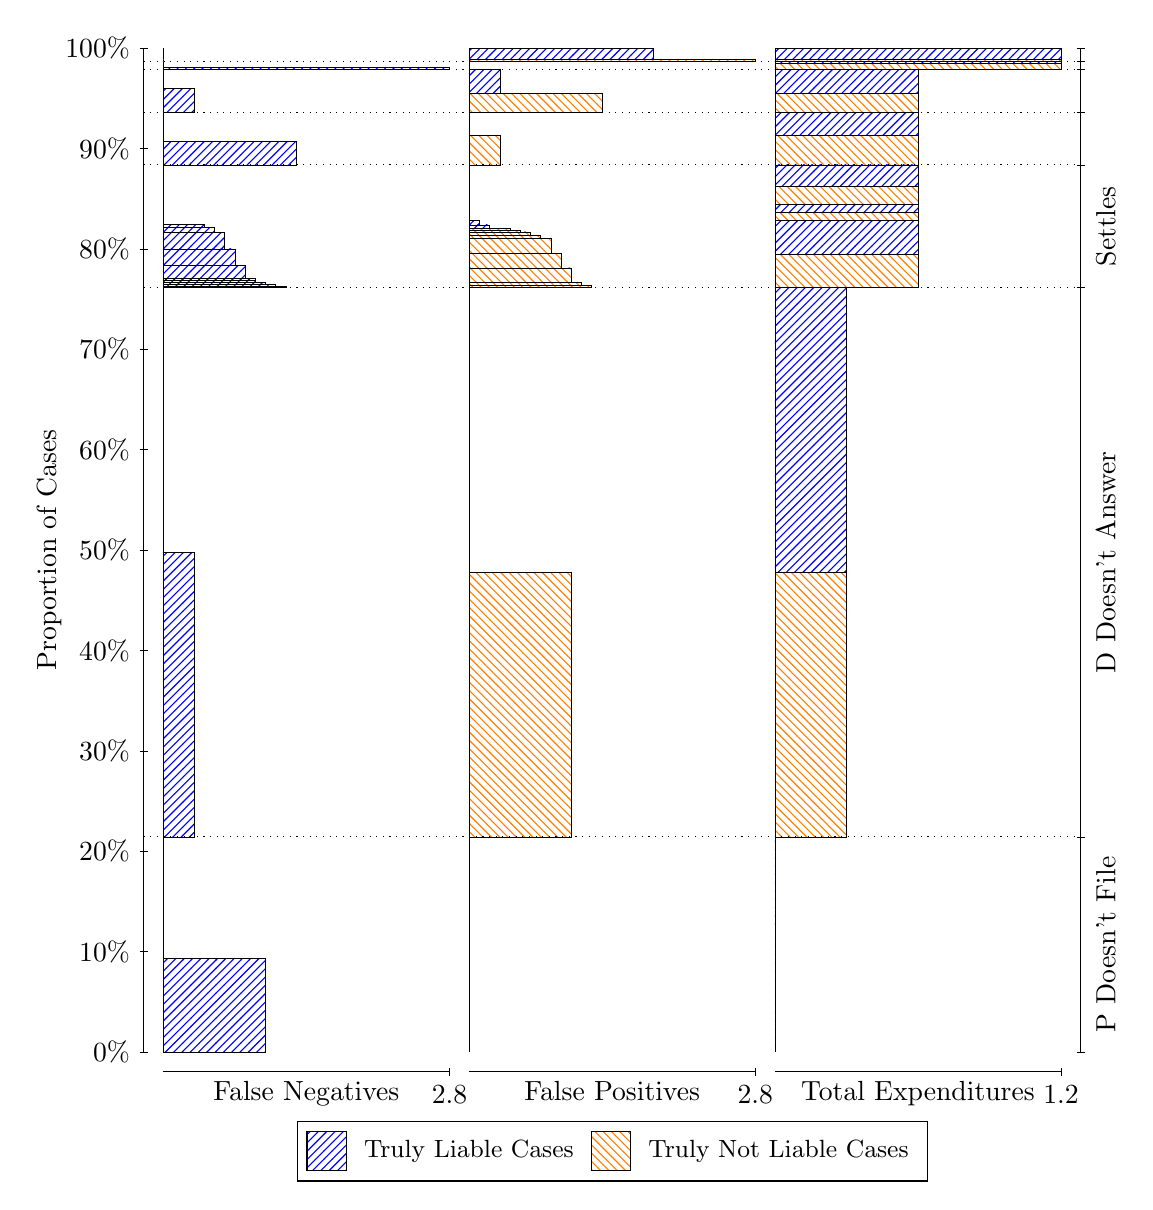
\begin{tikzpicture}
\draw[black, very thin] (1.5,1.75) -- (1.5,14.5);
\node[rotate=90, anchor=center] at (0.3, 8.125) {Proportion of Cases};
\draw[black, very thin] (1.45,1.75) -- (1.55,1.75);
\node[anchor=east] at (1.45, 1.75) {0\%};
\draw[black, very thin] (1.45,3.025) -- (1.55,3.025);
\node[anchor=east] at (1.45, 3.025) {10\%};
\draw[black, very thin] (1.45,4.3) -- (1.55,4.3);
\node[anchor=east] at (1.45, 4.3) {20\%};
\draw[black, very thin] (1.45,5.575) -- (1.55,5.575);
\node[anchor=east] at (1.45, 5.575) {30\%};
\draw[black, very thin] (1.45,6.85) -- (1.55,6.85);
\node[anchor=east] at (1.45, 6.85) {40\%};
\draw[black, very thin] (1.45,8.125) -- (1.55,8.125);
\node[anchor=east] at (1.45, 8.125) {50\%};
\draw[black, very thin] (1.45,9.4) -- (1.55,9.4);
\node[anchor=east] at (1.45, 9.4) {60\%};
\draw[black, very thin] (1.45,10.675) -- (1.55,10.675);
\node[anchor=east] at (1.45, 10.675) {70\%};
\draw[black, very thin] (1.45,11.95) -- (1.55,11.95);
\node[anchor=east] at (1.45, 11.95) {80\%};
\draw[black, very thin] (1.45,13.225) -- (1.55,13.225);
\node[anchor=east] at (1.45, 13.225) {90\%};
\draw[black, very thin] (1.45,14.5) -- (1.55,14.5);
\node[anchor=east] at (1.45, 14.5) {100\%};

\draw[black, very thin] (13.4,1.75) -- (13.4,14.5);
\draw[black, very thin] (13.35,1.75) -- (13.45,1.75);
\node[anchor=west] at (13.35, 1.75) {};
\draw[black, very thin] (13.35,4.4826) -- (13.45,4.4826);
\node[anchor=west] at (13.35, 4.4826) {};
\draw[black, very thin] (13.35,11.457) -- (13.45,11.457);
\node[anchor=west] at (13.35, 11.457) {};
\draw[black, very thin] (13.35,13.016) -- (13.45,13.016);
\node[anchor=west] at (13.35, 13.016) {};
\draw[black, very thin] (13.35,13.683) -- (13.45,13.683);
\node[anchor=west] at (13.35, 13.683) {};
\draw[black, very thin] (13.35,14.228) -- (13.45,14.228);
\node[anchor=west] at (13.35, 14.228) {};
\draw[black, very thin] (13.35,14.331) -- (13.45,14.331);
\node[anchor=west] at (13.35, 14.331) {};
\draw[black, very thin] (13.35,14.5) -- (13.45,14.5);
\node[anchor=west] at (13.35, 14.5) {};

\draw[black, very thin, pattern color=blue, pattern=north east lines] (1.75,1.75) rectangle (3.0476,2.9357);
\draw[black, very thin, pattern color=orange, pattern=north west lines] (1.75,2.9357) rectangle (1.75,4.4826);
\draw[black, very thin, pattern color=blue, pattern=north east lines] (1.75,4.4826) rectangle (2.1393,8.0953);
\draw[black, very thin, pattern color=orange, pattern=north west lines] (1.75,8.0953) rectangle (1.75,11.457);
\draw[black, very thin, pattern color=blue, pattern=north east lines] (1.75,11.457) rectangle (3.3071,11.475);
\draw[black, very thin, pattern color=blue, pattern=north east lines] (1.75,11.475) rectangle (3.1774,11.494);
\draw[black, very thin, pattern color=blue, pattern=north east lines] (1.75,11.494) rectangle (3.0476,11.528);
\draw[black, very thin, pattern color=blue, pattern=north east lines] (1.75,11.528) rectangle (2.9179,11.554);
\draw[black, very thin, pattern color=blue, pattern=north east lines] (1.75,11.554) rectangle (2.9179,11.571);
\draw[black, very thin, pattern color=blue, pattern=north east lines] (1.75,11.571) rectangle (2.7881,11.741);
\draw[black, very thin, pattern color=blue, pattern=north east lines] (1.75,11.741) rectangle (2.6583,11.95);
\draw[black, very thin, pattern color=blue, pattern=north east lines] (1.75,11.95) rectangle (2.5286,12.163);
\draw[black, very thin, pattern color=blue, pattern=north east lines] (1.75,12.163) rectangle (2.3988,12.218);
\draw[black, very thin, pattern color=blue, pattern=north east lines] (1.75,12.218) rectangle (2.269,12.265);
\draw[black, very thin, pattern color=orange, pattern=north west lines] (1.75,12.265) rectangle (1.75,13.016);
\draw[black, very thin, pattern color=blue, pattern=north east lines] (1.75,13.016) rectangle (3.4369,13.311);
\draw[black, very thin, pattern color=orange, pattern=north west lines] (1.75,13.311) rectangle (1.75,13.683);
\draw[black, very thin, pattern color=blue, pattern=north east lines] (1.75,13.683) rectangle (2.1393,13.987);
\draw[black, very thin, pattern color=orange, pattern=north west lines] (1.75,13.987) rectangle (1.75,14.228);
\draw[black, very thin, pattern color=blue, pattern=north east lines] (1.75,14.228) rectangle (5.3833,14.252);
\draw[black, very thin, pattern color=orange, pattern=north west lines] (1.75,14.252) rectangle (1.75,14.331);
\draw[black, very thin, pattern color=orange, pattern=north west lines] (1.75,14.331) rectangle (1.75,14.355);
\draw[black, very thin, pattern color=blue, pattern=north east lines] (1.75,14.355) rectangle (1.75,14.5);
\draw[black, very thin, pattern color=orange, pattern=north west lines] (5.6333,1.75) rectangle (5.6333,3.2969);
\draw[black, very thin, pattern color=blue, pattern=north east lines] (5.6333,3.2969) rectangle (5.6333,4.4826);
\draw[black, very thin, pattern color=orange, pattern=north west lines] (5.6333,4.4826) rectangle (6.931,7.8439);
\draw[black, very thin, pattern color=blue, pattern=north east lines] (5.6333,7.8439) rectangle (5.6333,11.457);
\draw[black, very thin, pattern color=orange, pattern=north west lines] (5.6333,11.457) rectangle (7.1905,11.487);
\draw[black, very thin, pattern color=orange, pattern=north west lines] (5.6333,11.487) rectangle (7.0607,11.525);
\draw[black, very thin, pattern color=orange, pattern=north west lines] (5.6333,11.525) rectangle (6.931,11.707);
\draw[black, very thin, pattern color=orange, pattern=north west lines] (5.6333,11.707) rectangle (6.8012,11.888);
\draw[black, very thin, pattern color=orange, pattern=north west lines] (5.6333,11.888) rectangle (6.6714,12.087);
\draw[black, very thin, pattern color=orange, pattern=north west lines] (5.6333,12.087) rectangle (6.5417,12.124);
\draw[black, very thin, pattern color=orange, pattern=north west lines] (5.6333,12.124) rectangle (6.4119,12.165);
\draw[black, very thin, pattern color=orange, pattern=north west lines] (5.6333,12.165) rectangle (6.2821,12.188);
\draw[black, very thin, pattern color=orange, pattern=north west lines] (5.6333,12.188) rectangle (6.1524,12.208);
\draw[black, very thin, pattern color=blue, pattern=north east lines] (5.6333,12.208) rectangle (5.8929,12.254);
\draw[black, very thin, pattern color=blue, pattern=north east lines] (5.6333,12.254) rectangle (5.7631,12.309);
\draw[black, very thin, pattern color=blue, pattern=north east lines] (5.6333,12.309) rectangle (5.6333,13.016);
\draw[black, very thin, pattern color=orange, pattern=north west lines] (5.6333,13.016) rectangle (6.0226,13.387);
\draw[black, very thin, pattern color=blue, pattern=north east lines] (5.6333,13.387) rectangle (5.6333,13.683);
\draw[black, very thin, pattern color=orange, pattern=north west lines] (5.6333,13.683) rectangle (7.3202,13.924);
\draw[black, very thin, pattern color=blue, pattern=north east lines] (5.6333,13.924) rectangle (6.0226,14.228);
\draw[black, very thin, pattern color=orange, pattern=north west lines] (5.6333,14.228) rectangle (5.6333,14.307);
\draw[black, very thin, pattern color=blue, pattern=north east lines] (5.6333,14.307) rectangle (5.6333,14.331);
\draw[black, very thin, pattern color=orange, pattern=north west lines] (5.6333,14.331) rectangle (9.2667,14.355);
\draw[black, very thin, pattern color=blue, pattern=north east lines] (5.6333,14.355) rectangle (7.969,14.5);
\draw[black, very thin, pattern color=orange, pattern=north west lines] (9.5167,1.75) rectangle (9.5167,3.2969);
\draw[black, very thin, pattern color=blue, pattern=north east lines] (9.5167,3.2969) rectangle (9.5167,4.4826);
\draw[black, very thin, pattern color=orange, pattern=north west lines] (9.5167,4.4826) rectangle (10.425,7.8439);
\draw[black, very thin, pattern color=blue, pattern=north east lines] (9.5167,7.8439) rectangle (10.425,11.457);
\draw[black, very thin, pattern color=orange, pattern=north west lines] (9.5167,11.457) rectangle (11.333,11.876);
\draw[black, very thin, pattern color=blue, pattern=north east lines] (9.5167,11.876) rectangle (11.333,12.315);
\draw[black, very thin, pattern color=orange, pattern=north west lines] (9.5167,12.315) rectangle (11.333,12.417);
\draw[black, very thin, pattern color=blue, pattern=north east lines] (9.5167,12.417) rectangle (11.333,12.514);
\draw[black, very thin, pattern color=orange, pattern=north west lines] (9.5167,12.514) rectangle (11.333,12.744);
\draw[black, very thin, pattern color=blue, pattern=north east lines] (9.5167,12.744) rectangle (11.333,13.016);
\draw[black, very thin, pattern color=orange, pattern=north west lines] (9.5167,13.016) rectangle (11.333,13.387);
\draw[black, very thin, pattern color=blue, pattern=north east lines] (9.5167,13.387) rectangle (11.333,13.683);
\draw[black, very thin, pattern color=orange, pattern=north west lines] (9.5167,13.683) rectangle (11.333,13.924);
\draw[black, very thin, pattern color=blue, pattern=north east lines] (9.5167,13.924) rectangle (11.333,14.228);
\draw[black, very thin, pattern color=orange, pattern=north west lines] (9.5167,14.228) rectangle (13.15,14.307);
\draw[black, very thin, pattern color=blue, pattern=north east lines] (9.5167,14.307) rectangle (13.15,14.331);
\draw[black, very thin, pattern color=orange, pattern=north west lines] (9.5167,14.331) rectangle (13.15,14.355);
\draw[black, very thin, pattern color=blue, pattern=north east lines] (9.5167,14.355) rectangle (13.15,14.5);
\draw[black, dotted] (1.5,4.4826) -- (13.4,4.4826);
\draw[black, dotted] (1.5,11.457) -- (13.4,11.457);
\draw[black, dotted] (1.5,13.016) -- (13.4,13.016);
\draw[black, dotted] (1.5,13.683) -- (13.4,13.683);
\draw[black, dotted] (1.5,14.228) -- (13.4,14.228);
\draw[black, dotted] (1.5,14.331) -- (13.4,14.331);
\draw[black, very thin] (1.75,1.5) -- (5.3833,1.5);
\node[anchor=north] at (3.5667, 1.5) {False Negatives};
\draw[black, very thin] (5.3833,1.45) -- (5.3833,1.55);
\node[anchor=north] at (5.3833, 1.45) {2.8};

\draw[black, very thin] (5.6333,1.5) -- (9.2667,1.5);
\node[anchor=north] at (7.45, 1.5) {False Positives};
\draw[black, very thin] (9.2667,1.45) -- (9.2667,1.55);
\node[anchor=north] at (9.2667, 1.45) {2.8};

\draw[black, very thin] (9.5167,1.5) -- (13.15,1.5);
\node[anchor=north] at (11.333, 1.5) {Total Expenditures};
\draw[black, very thin] (13.15,1.45) -- (13.15,1.55);
\node[anchor=north] at (13.15, 1.45) {1.2};

\node[black, centered, rotate=90] at (13.72, 3.1163) {P Doesn't File};
\node[black, centered, rotate=90] at (13.72, 7.9696) {D Doesn't Answer};
\node[black, centered, rotate=90] at (13.72, 12.236) {Settles};





\draw (7.449999999999999,1.5) node[draw=none] (baseCoordinate) {};
\begin{scope}[align=center]
        \matrix[scale=0.5, draw=black, below=0.5cm of baseCoordinate, nodes={draw}, column sep=0.1cm]{
            \node[rectangle, draw, minimum width=0.5cm, minimum height=0.5cm, pattern=north east lines, pattern color=blue] {}; &
            \node[draw=none, font=\small] (B) {Truly Liable Cases}; &
            \node[rectangle, draw, minimum width=0.5cm, minimum height=0.5cm, pattern=north west lines, pattern color=orange] {}; &
            \node[draw=none, font=\small] (B) {Truly Not Liable Cases}; \\
            };
\end{scope}

\end{tikzpicture}
\end{document}